\documentclass[tikz,border=6pt]{standalone}
\usepackage[utf8]{inputenc}
\usepackage[T1]{fontenc}
\usepackage{amsmath,amssymb,bm}
\usepackage{mathptmx}
\usetikzlibrary{arrows.meta,positioning,calc,decorations.pathmorphing,shapes.geometric}
\begin{document}
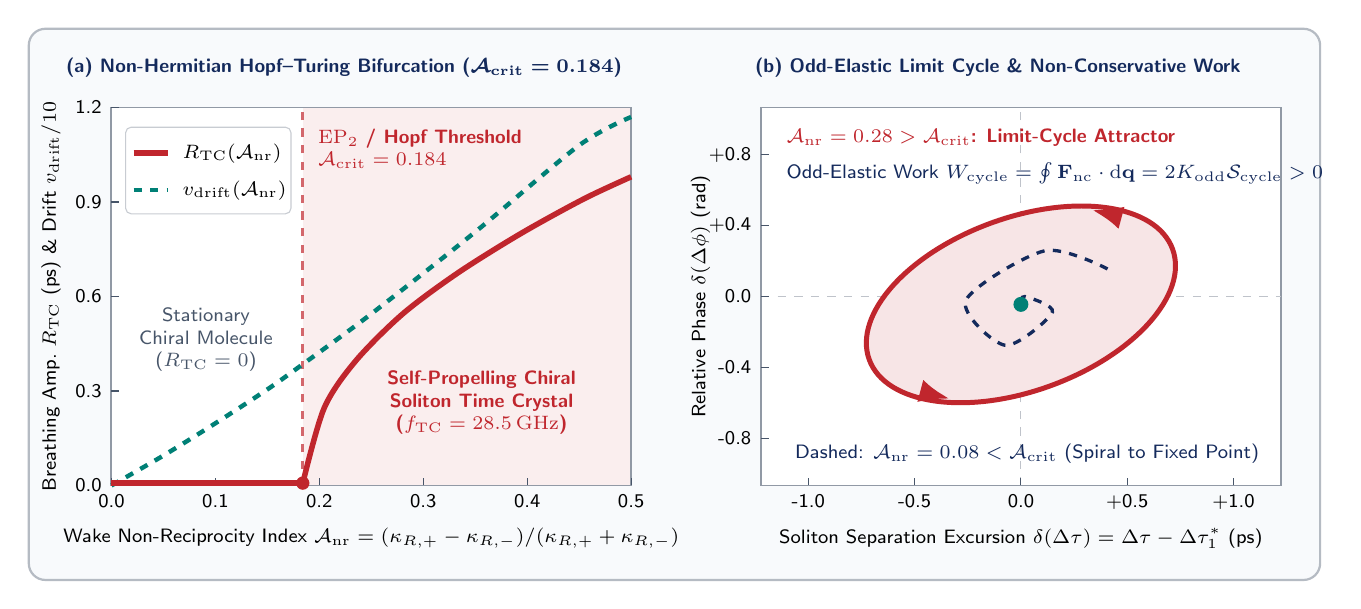
\begin{tikzpicture}[font=\sffamily\small, >=Latex]
  \definecolor{navy}{RGB}{20,42,92}
  \definecolor{tealcol}{RGB}{0,128,118}
  \definecolor{crimson}{RGB}{192,38,45}
  \definecolor{amber}{RGB}{217,119,6}
  \definecolor{slate}{RGB}{71,85,105}
  \definecolor{softbg}{RGB}{248,250,252}

  \fill[softbg, rounded corners=6pt] (0,0) rectangle (16.4, 7.0);
  \draw[slate!40, line width=0.8pt, rounded corners=6pt] (0,0) rectangle (16.4, 7.0);

  % ---------------- PANEL (a) ----------------
  \node[anchor=north west, font=\sffamily\bfseries\scriptsize, text=navy] at (0.35, 6.75)
    {(a) Non-Hermitian Hopf--Turing Bifurcation ($\bm{\mathcal{A}_{\mathrm{crit}} = 0.184}$)};

  \begin{scope}[shift={(1.05, 1.20)}]
    \fill[white] (0,0) rectangle (6.6, 4.8);
    % Shaded Time-Crystal region for A_nr > 0.184 (x = 2.43 to 6.6)
    \fill[crimson!8] (2.43, 0) rectangle (6.6, 4.8);
    \draw[crimson!70, dashed, line width=1.1pt] (2.43, 0) -- (2.43, 4.8);
    \node[anchor=north west, font=\sffamily\scriptsize\bfseries, text=crimson, align=left] at (2.50, 4.65)
      {$\mathrm{EP}_2$ / Hopf Threshold\\$\mathcal{A}_{\mathrm{crit}} = 0.184$};

    \draw[slate!60, line width=0.7pt] (0,0) rectangle (6.6, 4.8);

    % X-axis ticks (A_nr from 0 to 0.50 -> 6.6 units => 13.2 units per A_nr)
    \foreach \a/\x in {0.0/0.0, 0.1/1.32, 0.2/2.64, 0.3/3.96, 0.4/5.28, 0.5/6.60} {
      \draw[slate] (\x, 0) -- (\x, 0.1);
      \node[below, font=\sffamily\scriptsize] at (\x, 0) {\a};
    }
    \node[below, font=\sffamily\scriptsize] at (3.3, -0.42)
      {Wake Non-Reciprocity Index $\mathcal{A}_{\mathrm{nr}} = (\kappa_{R,+} - \kappa_{R,-})/(\kappa_{R,+} + \kappa_{R,-})$};

    % Y-axis ticks (0 to 1.2)
    \foreach \y/\lbl in {0.0/0.0, 1.2/0.3, 2.4/0.6, 3.6/0.9, 4.8/1.2} {
      \draw[slate] (0, \y) -- (0.1, \y);
      \node[left, font=\sffamily\scriptsize] at (0, \y) {\lbl};
    }
    \node[rotate=90, above, font=\sffamily\scriptsize] at (-0.52, 2.4)
      {Breathing Amp.\ $R_{\mathrm{TC}}$ (ps) \& Drift $v_{\mathrm{drift}}/10$};

    % Curve 1: Chiral Drift Velocity v_drift / 10 (teal dashed)
    \draw[tealcol, dashed, line width=1.6pt, smooth] plot coordinates {
      (0.0, 0.0) (0.66, 0.38) (1.32, 0.79) (1.98, 1.22) (2.43, 1.54)
      (3.30, 2.18) (4.62, 3.22) (5.94, 4.32) (6.60, 4.68)
    };

    % Curve 2: Time-Crystal Breathing Amplitude R_TC (crimson solid, zero below A_crit=2.43)
    \draw[crimson, line width=2.0pt] (0.0, 0.03) -- (2.43, 0.03);
    \draw[crimson, line width=2.0pt, smooth] plot coordinates {
      (2.43, 0.03) (2.70, 0.98) (3.10, 1.58) (3.70, 2.18) (4.40, 2.70)
      (5.20, 3.20) (6.00, 3.64) (6.60, 3.92)
    };
    \filldraw[crimson] (2.43, 0.03) circle (2.2pt);

    % Legend box at top-left
    \fill[white, draw=slate!30, rounded corners=2pt] (0.18, 3.45) rectangle (2.28, 4.55);
    \draw[crimson, line width=2.0pt] (0.28, 4.22) -- (0.72, 4.22);
    \node[anchor=west, font=\sffamily\scriptsize] at (0.78, 4.22) {$R_{\mathrm{TC}}(\mathcal{A}_{\mathrm{nr}})$};
    \draw[tealcol, dashed, line width=1.6pt] (0.28, 3.75) -- (0.72, 3.75);
    \node[anchor=west, font=\sffamily\scriptsize] at (0.78, 3.75) {$v_{\mathrm{drift}}(\mathcal{A}_{\mathrm{nr}})$};

    \node[font=\sffamily\scriptsize, text=slate, align=center] at (1.2, 1.85)
      {Stationary\\Chiral Molecule\\($R_{\mathrm{TC}} = 0$)};
    \node[font=\sffamily\scriptsize\bfseries, text=crimson, align=center] at (4.7, 1.05)
      {Self-Propelling Chiral\\Soliton Time Crystal\\($f_{\mathrm{TC}} = 28.5\,\mathrm{GHz}$)};
  \end{scope}

  % ---------------- PANEL (b) ----------------
  \node[anchor=north west, font=\sffamily\bfseries\scriptsize, text=navy] at (9.10, 6.75)
    {(b) Odd-Elastic Limit Cycle \& Non-Conservative Work};

  \begin{scope}[shift={(9.3, 1.20)}]
    \fill[white] (0,0) rectangle (6.6, 4.8);
    \draw[slate!60, line width=0.7pt] (0,0) rectangle (6.6, 4.8);

    % Center axes
    \draw[slate!35, dashed] (0, 2.4) -- (6.6, 2.4);
    \draw[slate!35, dashed] (3.3, 0) -- (3.3, 4.8);

    \node[below, font=\sffamily\scriptsize] at (3.3, -0.42)
      {Soliton Separation Excursion $\delta(\Delta\tau) = \Delta\tau - \Delta\tau_1^*$ (ps)};
    \node[rotate=90, above, font=\sffamily\scriptsize] at (-0.52, 2.4)
      {Relative Phase $\delta(\Delta\phi)$ (rad)};

    % Ticks
    \foreach \x/\lbl in {0.6/-1.0, 1.95/-0.5, 3.3/0.0, 4.65/+0.5, 6.0/+1.0} {
      \draw[slate] (\x, 0) -- (\x, 0.1);
      \node[below, font=\sffamily\scriptsize] at (\x, 0) {\lbl};
    }
    \foreach \y/\lbl in {0.6/-0.8, 1.5/-0.4, 2.4/0.0, 3.3/+0.4, 4.2/+0.8} {
      \draw[slate] (0, \y) -- (0.1, \y);
      \node[left, font=\sffamily\scriptsize] at (0, \y) {\lbl};
    }

    % Shaded limit cycle ellipse for A_nr = 0.28 > A_crit
    \fill[crimson!12, rotate around={20:(3.3,2.3)}] (3.3, 2.3) ellipse (2.05 and 1.10);
    \draw[crimson, line width=1.8pt, rotate around={20:(3.3,2.3)}] (3.3, 2.3) ellipse (2.05 and 1.10);

    % Directional arrows on limit cycle showing chiral circulation
    \draw[->, crimson, line width=1.8pt] (4.50, 3.42) -- (4.20, 3.50);
    \draw[->, crimson, line width=1.8pt] (2.10, 1.18) -- (2.40, 1.10);

    % Damped spiral for A_nr = 0.08 < A_crit (navy dashed)
    \draw[navy, dashed, line width=1.2pt, smooth] plot coordinates {
      (4.4, 2.75) (3.6, 2.98) (2.6, 2.35) (3.1, 1.78) (3.7, 2.20) (3.35, 2.40) (3.3, 2.3)
    };
    \filldraw[tealcol] (3.3, 2.3) circle (2.5pt);

    % Annotations in top/bottom bands
    \node[anchor=north west, font=\sffamily\scriptsize\bfseries, text=crimson] at (0.20, 4.65)
      {$\mathcal{A}_{\mathrm{nr}} = 0.28 > \mathcal{A}_{\mathrm{crit}}$: Limit-Cycle Attractor};
    \node[anchor=north west, font=\sffamily\scriptsize, text=navy] at (0.20, 4.22)
      {Odd-Elastic Work $W_{\mathrm{cycle}} = \oint \mathbf{F}_{\mathrm{nc}}\cdot \mathrm{d}\mathbf{q} = 2K_{\mathrm{odd}}\mathcal{S}_{\mathrm{cycle}} > 0$};
    \node[anchor=south east, font=\sffamily\scriptsize, text=navy] at (6.45, 0.16)
      {Dashed: $\mathcal{A}_{\mathrm{nr}} = 0.08 < \mathcal{A}_{\mathrm{crit}}$ (Spiral to Fixed Point)};
  \end{scope}
\end{tikzpicture}

\end{document}
